\section{Wednesday for MAT4002}\index{Monday_lecture}
\subsection{The fundamental group}
\paragraph{Revewing}
One example for Homotopy relative to $\{0,1\}$ is illustrated in Fig.(\ref{Fig:11:5})
\begin{figure}[H]
\centering
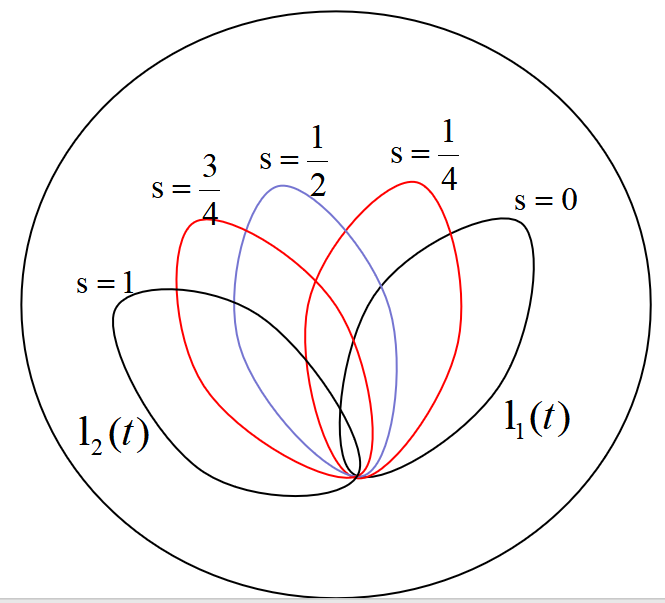
\includegraphics[width=0.3\textwidth]{week11/relative.png}
\caption{Example of homotopy relative to $\{0,1\}$}
\end{figure}
It's \emph{essential} to study homotopy relative to $\{0,1\}$.
For example, given a torus with a loop $\ell_1(t)$ and a base point $b$.
We want to distinguish $\ell_1(t)$ and $\ell_2(t)$ as shown in Fig.(\ref{Fig:11:6}):
\begin{figure}[H]
\centering
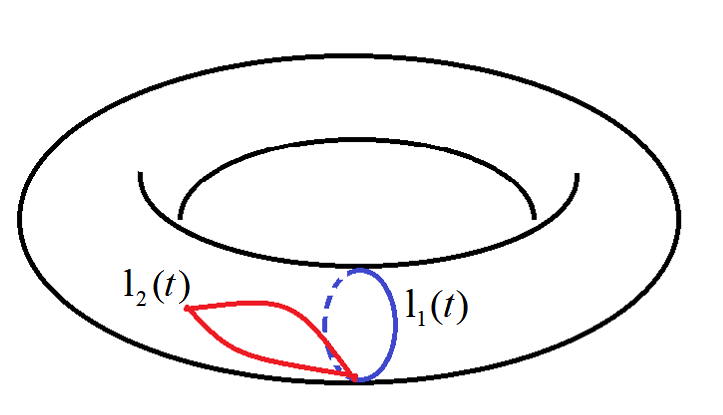
\includegraphics[width=0.4\textwidth]{week11/twolooptorus.png}
\caption{Two loops on a torus}
\label{Fig:11:6}
\end{figure}
Obviously there should be something different between $\ell_1(t)$ and $\ell_2(t)$.
``Relative to$\{0,1\}$ is essential'', sicne if we get rid of this condition, all loops are homotopic to the constant map $c_b(t)=b$. See the graphic illustration in Fig.(\ref{Fig:11:7}):
\begin{figure}[H]
	\centering{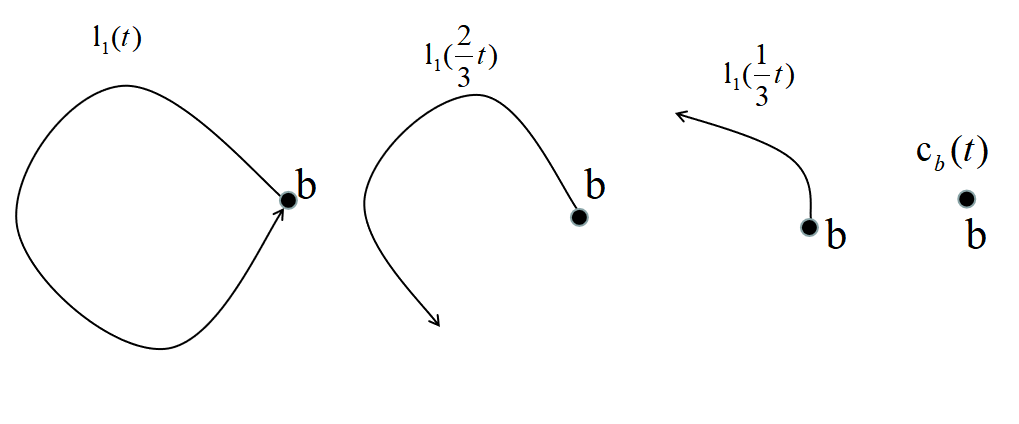
\includegraphics[width=0.4\textwidth]{week11/homtoconst.png}}
	\caption{homotopy between any loop and constant map}
	\label{fig: 1:7}
\end{figure}
In this case, $\ell\simeq c_b$ for any loop $\ell$, there is only one trivial element $\{[c_b]\}$ in $\pi_1(X,b)$.

That's the reason why we define $\pi_1(X,b)$ as the collection of homotopy classes \emph{relative to $\{0,1\}$} based at $b$ in $X$.
\begin{proposition}
Let $[\cdot]$ denote the homotopy class of loops relative to $\{0,1\}$ based at $b$, and define the operation
\begin{align*}
[\ell]*[\ell']&=[\ell\cdot\ell']\\
\end{align*}
Then $(\pi_1(X,b),*)$ forms a group, where
\[
\pi_1(X,b) := \{[\ell]\mid \ell:[0,1]\to X\text{ denotes loops based at $b$}\} 
\]
\end{proposition}
\begin{proof}
\begin{enumerate}
\item
Well-definedness:
Suppose that $u\sim u'$ and $v\sim v'$, it suffices to show $u\cdot v\simeq u'\cdot v'$.
Consider the given homotopies $H:u\simeq u'$, $K:v\simeq v'$.
Construct a new homotopy $L:I\times I\to X$ by
\[
L(t,s)=\left\{
\begin{aligned}
H(2t,s),&\quad 0\le t\le 1/2\\
K(2t-1,s),&\quad 1/2\le t\le 1
\end{aligned}
\right.
\] 
The diagram below explains the ideas for constructing $L$.
The plane denote the set $I\times I$, and the labels characterize the images of each point of $I\times I$ under $L$.
\begin{figure}[H]
	\centering{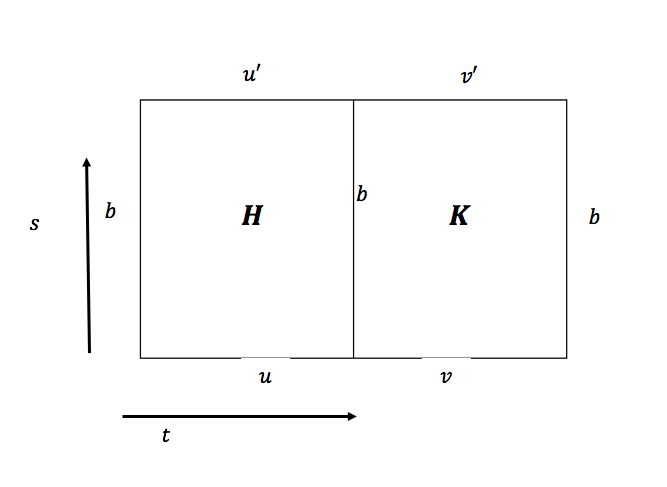
\includegraphics[width=0.6\textwidth]{week11/fig_11_7.png}}
	\label{Fig:11:7}
\end{figure}
Therefore, $u\cdot v\simeq u'\cdot v'$.
\item
Associate: $(u\cdot v)\cdot w\simeq u\cdot(v\cdot w)$

Note that $(u\cdot v)\cdot w$ and $u\cdot(v\cdot w)$ are essentially different loops. Although they go with the same path, they are with different speeds. Generally speaking, the loop $(u\cdot v)\cdot w$ travels $u,v$ using $1/4$ seconds, and $w$ in $1/2$ seconds; but the loop $u\cdot(v\cdot w)$ travels $u$ in $1/2$ seconds, and then $v,w$ in $1/4$ seconds.

We want to construct a homotopy that describes the loop changes from $u\cdot(v\cdot w)$ to $(u\cdot v)\cdot w$. A graphic illustration is given below:
\begin{figure}[H]
	\centering{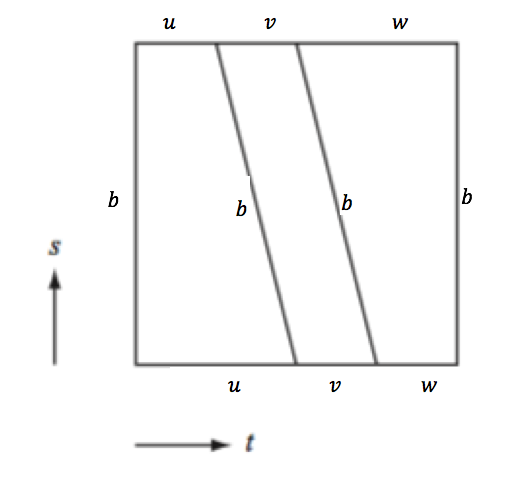
\includegraphics[width=0.4\textwidth]{week11/fig_11_8.png}}
	\label{Fig:11:8}
\end{figure}
An explicit homotopy $H:I\times I\to X$ is given below:
\[
H(t,s) = \left\{
\begin{aligned}
u(4t/(2-s)),&\quad 0\le t\le 1/2-1/4s\\
v(4t - 2+s),&\quad 1/2 - 1/4s\le t\le 3/4 - 1/4s\\
w(4t - 3+s/(1+s)),&\quad 3/4 - 1/4s\le t\le 1
\end{aligned}
\right.
\]
Therefore,
\[
[u]*([v]*[w])=([u]*[v])*[w]
\]
\item
Intuitively, the identity should be the constant map, i.e., let $c_b:I\to X$ by $c_b(t) = b,\forall t$, and let $\ell = [c_b]$, it suffices to show
\[
[c_b]*[\ell]=[\ell]*[c_b]=[\ell]
\Longleftrightarrow
[c_b\cdot\ell]=[\ell\cdot c_b]=[\ell]
\]
Or equivalently,
\[
c_b\cdot\ell\simeq\ell,\quad
\ell\cdot c_b\simeq \ell
\]
The graphic homotopy is shown below. (You should have been understood this diagram)
\begin{figure}[H]
	\centering{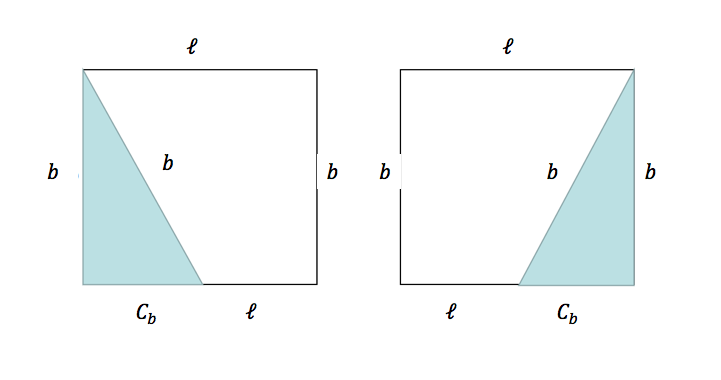
\includegraphics[width=0.6\textwidth]{week11/fig_11_9.png}}
	\label{Fig:11:9}
\end{figure}
\item
Inverse: the inverse of $[u]$, where $u$ is a loop, should be $[u']$, where $u'$ is the reverse of the traveling of $u$.
Therefore, for all $u:I\to X$ (loop based at $b$), define $u^{-1}:I\to X$ by $u^{-1}(t)=u(1-t)$.
Note that
\[
\begin{array}{ll}
[u]*[u^{-1}]=[u\cdot u^{-1}],
&
e = [c_b] 
\end{array}
\]
It suffices to show $u\cdot u^{-1}\simeq c_b$ and $u^{-1}\cdot u\simeq c_b$:

The homotopy below gives $u\cdot u^{-1}\simeq c_b$, and the $u^{-1}\cdot u\simeq c_b$ follows similarly.
\[
H(t,s)=\left\{
\begin{aligned}
u(2t(1-s)),&\quad 0\le t\le 1/2\\
u((2-2t)(1-s)),&\quad 1/2\le t\le 1
\end{aligned}
\right.
\]
The graphic illustration is given below:
\begin{figure}[H]
	\centering{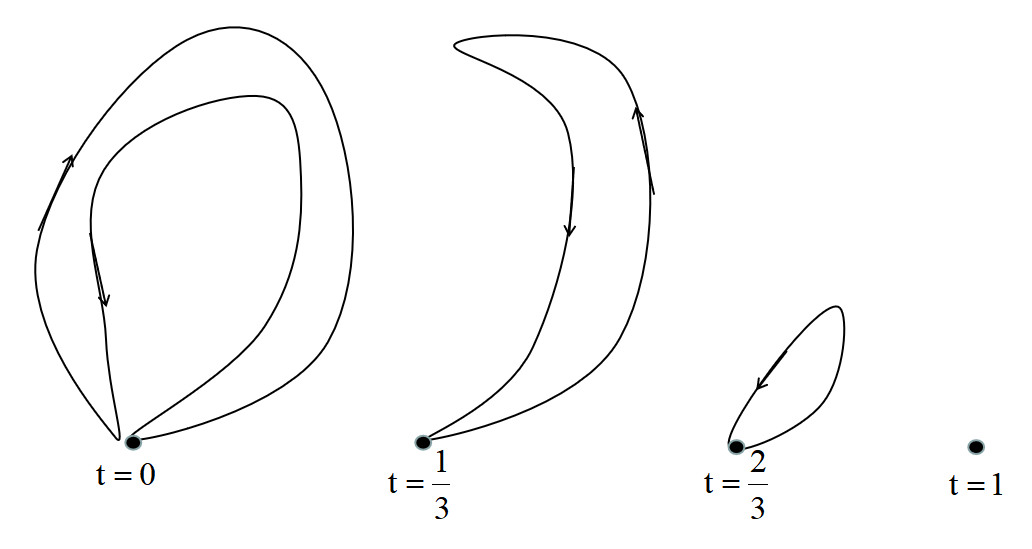
\includegraphics[width=0.6\textwidth]{week11/homotopy3.png}}
	\label{fig: 1:10}
\end{figure}
\end{enumerate}
\end{proof}
\begin{remark}
Note that the figure below does not define a homotopy from $u\cdot u^{-1}$ to $c_b$!
\begin{figure}[H]
	\centering{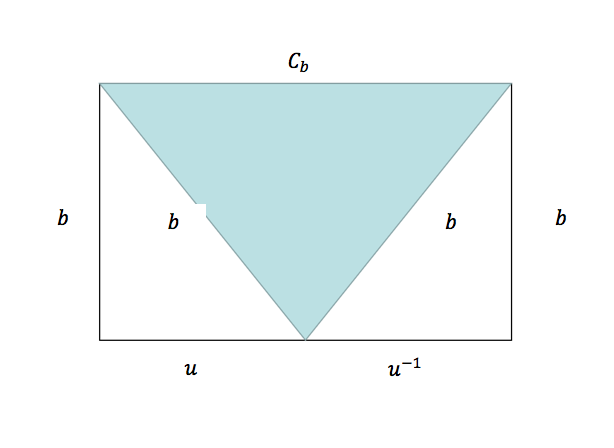
\includegraphics[width=0.6\textwidth]{week11/fig_11_10.png}}
\end{figure}
The reason is that for the upper part, as $s\to1$, the time for traveling $u$ and $u^{-1}$ becomes very small, i.e., a particle has to pass $u$ and $u^{-1}$ in infinitely small time, which is not well-defined.
\end{remark}


\begin{example}
The reason why $\pi_1(\mathbb{R}^2,b) = \{e\}$ is trivial:
\begin{itemize}
\item
For any $u:I\to\mathbb{R}^2$ with $u(0)=u(1)=b$, consider the homotopy 
\[
H(t,s) = (1-s)u(t)+sb.
\]
Therefore, $u\simeq c_b$ for any loop $u$ based at $b$.
Check the diagram below for graphic illustration of this homotopy.
\begin{figure}[H]
	\centering{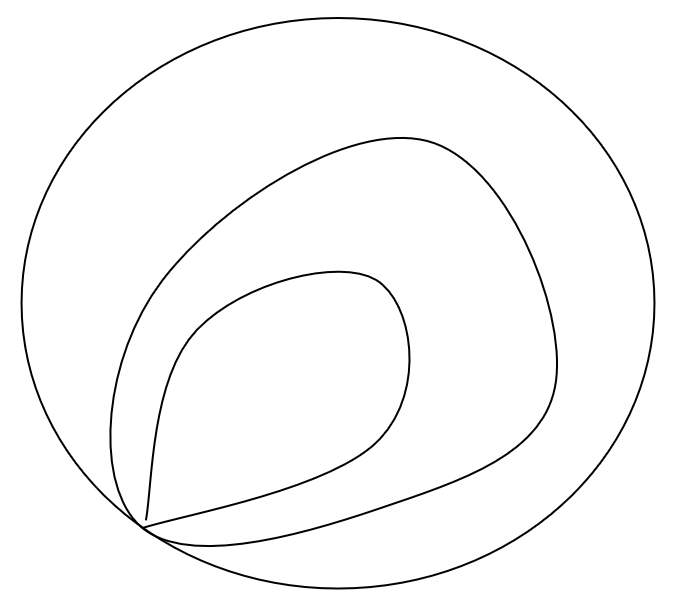
\includegraphics[width=0.3\textwidth]{week11/homotopy5.png}}
\end{figure}
More generally, if $X\simeq\{x\}$ is contractible, then $\pi_1(X,b)=\{e\}$.
The same argument cannot work for $(\mathbb{R}^2 \{0\}, \bm b)$, since the mapping 
$H:\mathbb{R}^2\setminus\{0\}\times I\to \mathbb{R}^2\setminus\{0\}$ with $H(\bm t,s) = (1-s)u(\bm t) + s\bm b$ is not well-defined. In particular, the value $H(s,t)$ may hit the origin $\bm0$.
\end{itemize}
However, $\pi_1(S^1,1)$ is non-trivial. 
We cannot deform the loop in $S^1$ into a constant loop.
We will see that $\pi_1(S^1,1) \cong\mathbb{Z}$.
\end{example}




\begin{proposition}
If $b,b'$ are path-connected in $X$, then $\pi_1(X,b)\cong\pi_1(X,b')$.
\end{proposition}
\begin{proof}
Let $w$ be a path from $b$ to $b'$, and define
\[
\begin{array}{ll}
w_{\#}:&\pi_1(X,b)\to\pi_1(X,b')\\
\text{with}&[\ell]\mapsto[w^{-1}\ell w]
\end{array}
\]
\begin{enumerate}
\item
Well-definedness: Check that $\ell\simeq\ell'$ implies $w^{-1}\ell w\simeq w^{-1}\ell' w$.
See the figure below for graphic illustration.
\begin{figure}[H]
	\centering{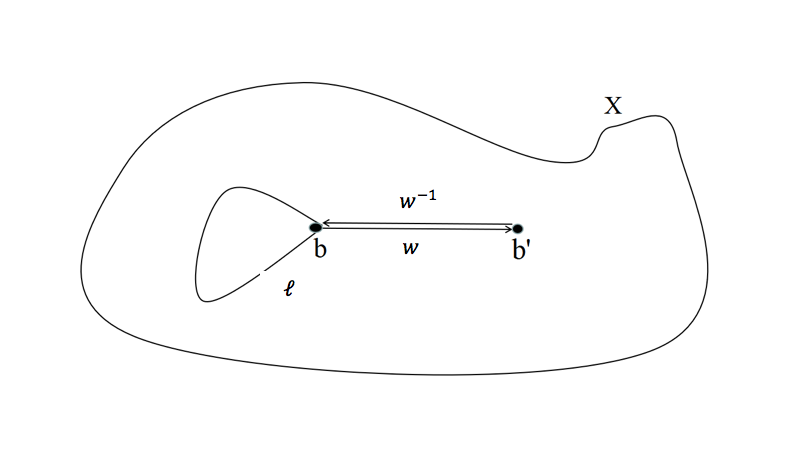
\includegraphics[width=0.6\textwidth]{week11/fig_11_11.png}}
	\label{fig: 1:14}
\end{figure}
\item
$w_{\#}$ is a homomorphism:
\begin{subequations}
\begin{align}
	w_{\#}([\ell_1]) \cdot w_{\#}([\ell_2]) =& [w^{-1}\cdot \ell_1 w] \cdot [w^{-1}\cdot \ell_2 w]\\
	=& [w^{-1}\cdot \ell_1 \ell_2 w]\label{Eq:11:4:b}\\
    =& w_{\#}([\ell_1 \ell_2])
\end{align}
where (\ref{Eq:11:4:b}) is because that $w\cdot w^{-1}=c_b$.
\end{subequations}
\item
And $w_{\#}$ is also injective. If loops $\ell_1$, $\ell_2$ are such that $w_{\#}(\ell_1) = w_{\#}(\ell_2)$, then
\[
	[w^{-1}\ell_1 w] = [w^{-1} \ell_2 w],
\]
which follows that
\begin{equation}\label{Eq:11:5}
 [\ell_1] = [w][w^{-1}\ell_1 w][w^{-1}] =  [w][w^{-1} \ell_2 w][w^{-1}] = [\ell_2]
\end{equation}
\item
Finally, $w_{\#}$ is surjective, because for any $u\in \pi_1(X, b')$,  let $v = wuw^{-1}$, then $v$ is based at $b$, so $[v]\in \pi_1(X, b)$,  and $w_{\#}(v) = [u]$.
Therefore $w_{\#}$ is surjective. 
\end{enumerate}
In conclusion, $w_{\#}$ is a group isomorphism between $\pi_1(X, b)$ and $\pi_1(X, b')$.
\end{proof}

\begin{remark}
In (\ref{Eq:11:5}) we extended the meaning of $[\ell]$ to allow $\ell$ to be a path, and the equivalence class is defined by the relation ``$\sim$'': $\ell_1\sim \ell_2$ iff they are homotopic relative to $\{0,1\}$. The multiplication rules are defined similarly.
\end{remark}



















